\documentclass[a4paper]{article}

\usepackage[utf8]{inputenc}
\usepackage[T1]{fontenc}

\usepackage{booktabs}
\usepackage{amsmath}

\usepackage{tikz}
\usetikzlibrary{} 

\title{Find range limited by conditions}
\date{}
\author{}
\begin{document}
\maketitle
\section{Problem}
\noindent
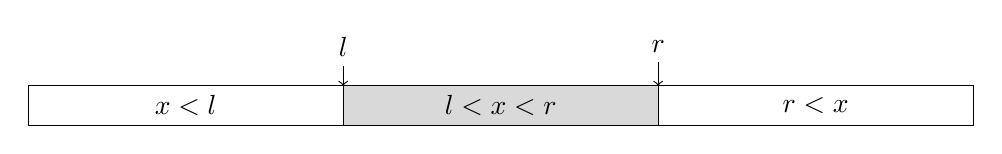
\begin{tikzpicture}[scale=1,auto=center]
  \draw (0,0) rectangle node{$x < l$} (4,.5);
  \draw[fill=black!15] (4,0) rectangle node{$l < x < r$} (8,.5);
  \draw (8,0) rectangle node{$r < x$} (12,.5);
  \node (l) at (4,1) {$l$};
  \node (r) at (8,1) {$r$};
  \draw[->] (l) -- (4,.5);
  \draw[->] (r) -- (8,.5);
\end{tikzpicture}

\vspace{1cm}

\noindent
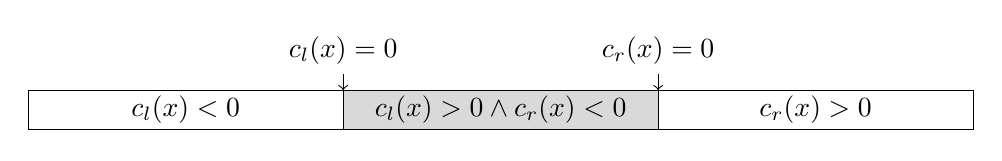
\begin{tikzpicture}[scale=1,auto=center]
  \draw (0,0) rectangle node{$c_l(x) < 0$} (4,.5);
  \draw[fill=black!15] (4,0) rectangle node{$c_l(x) > 0 \wedge c_r(x) < 0$} (8,.5);
  \draw (8,0) rectangle node{$c_r(x) > 0$} (12,.5);
  \node (l) at (4,1) {$c_l(x)=0$};
  \node (r) at (8,1) {$c_r(x)=0$};
  \draw[->] (l) -- (4,.5);
  \draw[->] (r) -- (8,.5);
\end{tikzpicture}
\end{document}
